\chapter{Case Study: Certified Concurrent OS Kernel}
\label{chap:conkernel}

\begin{figure*}
%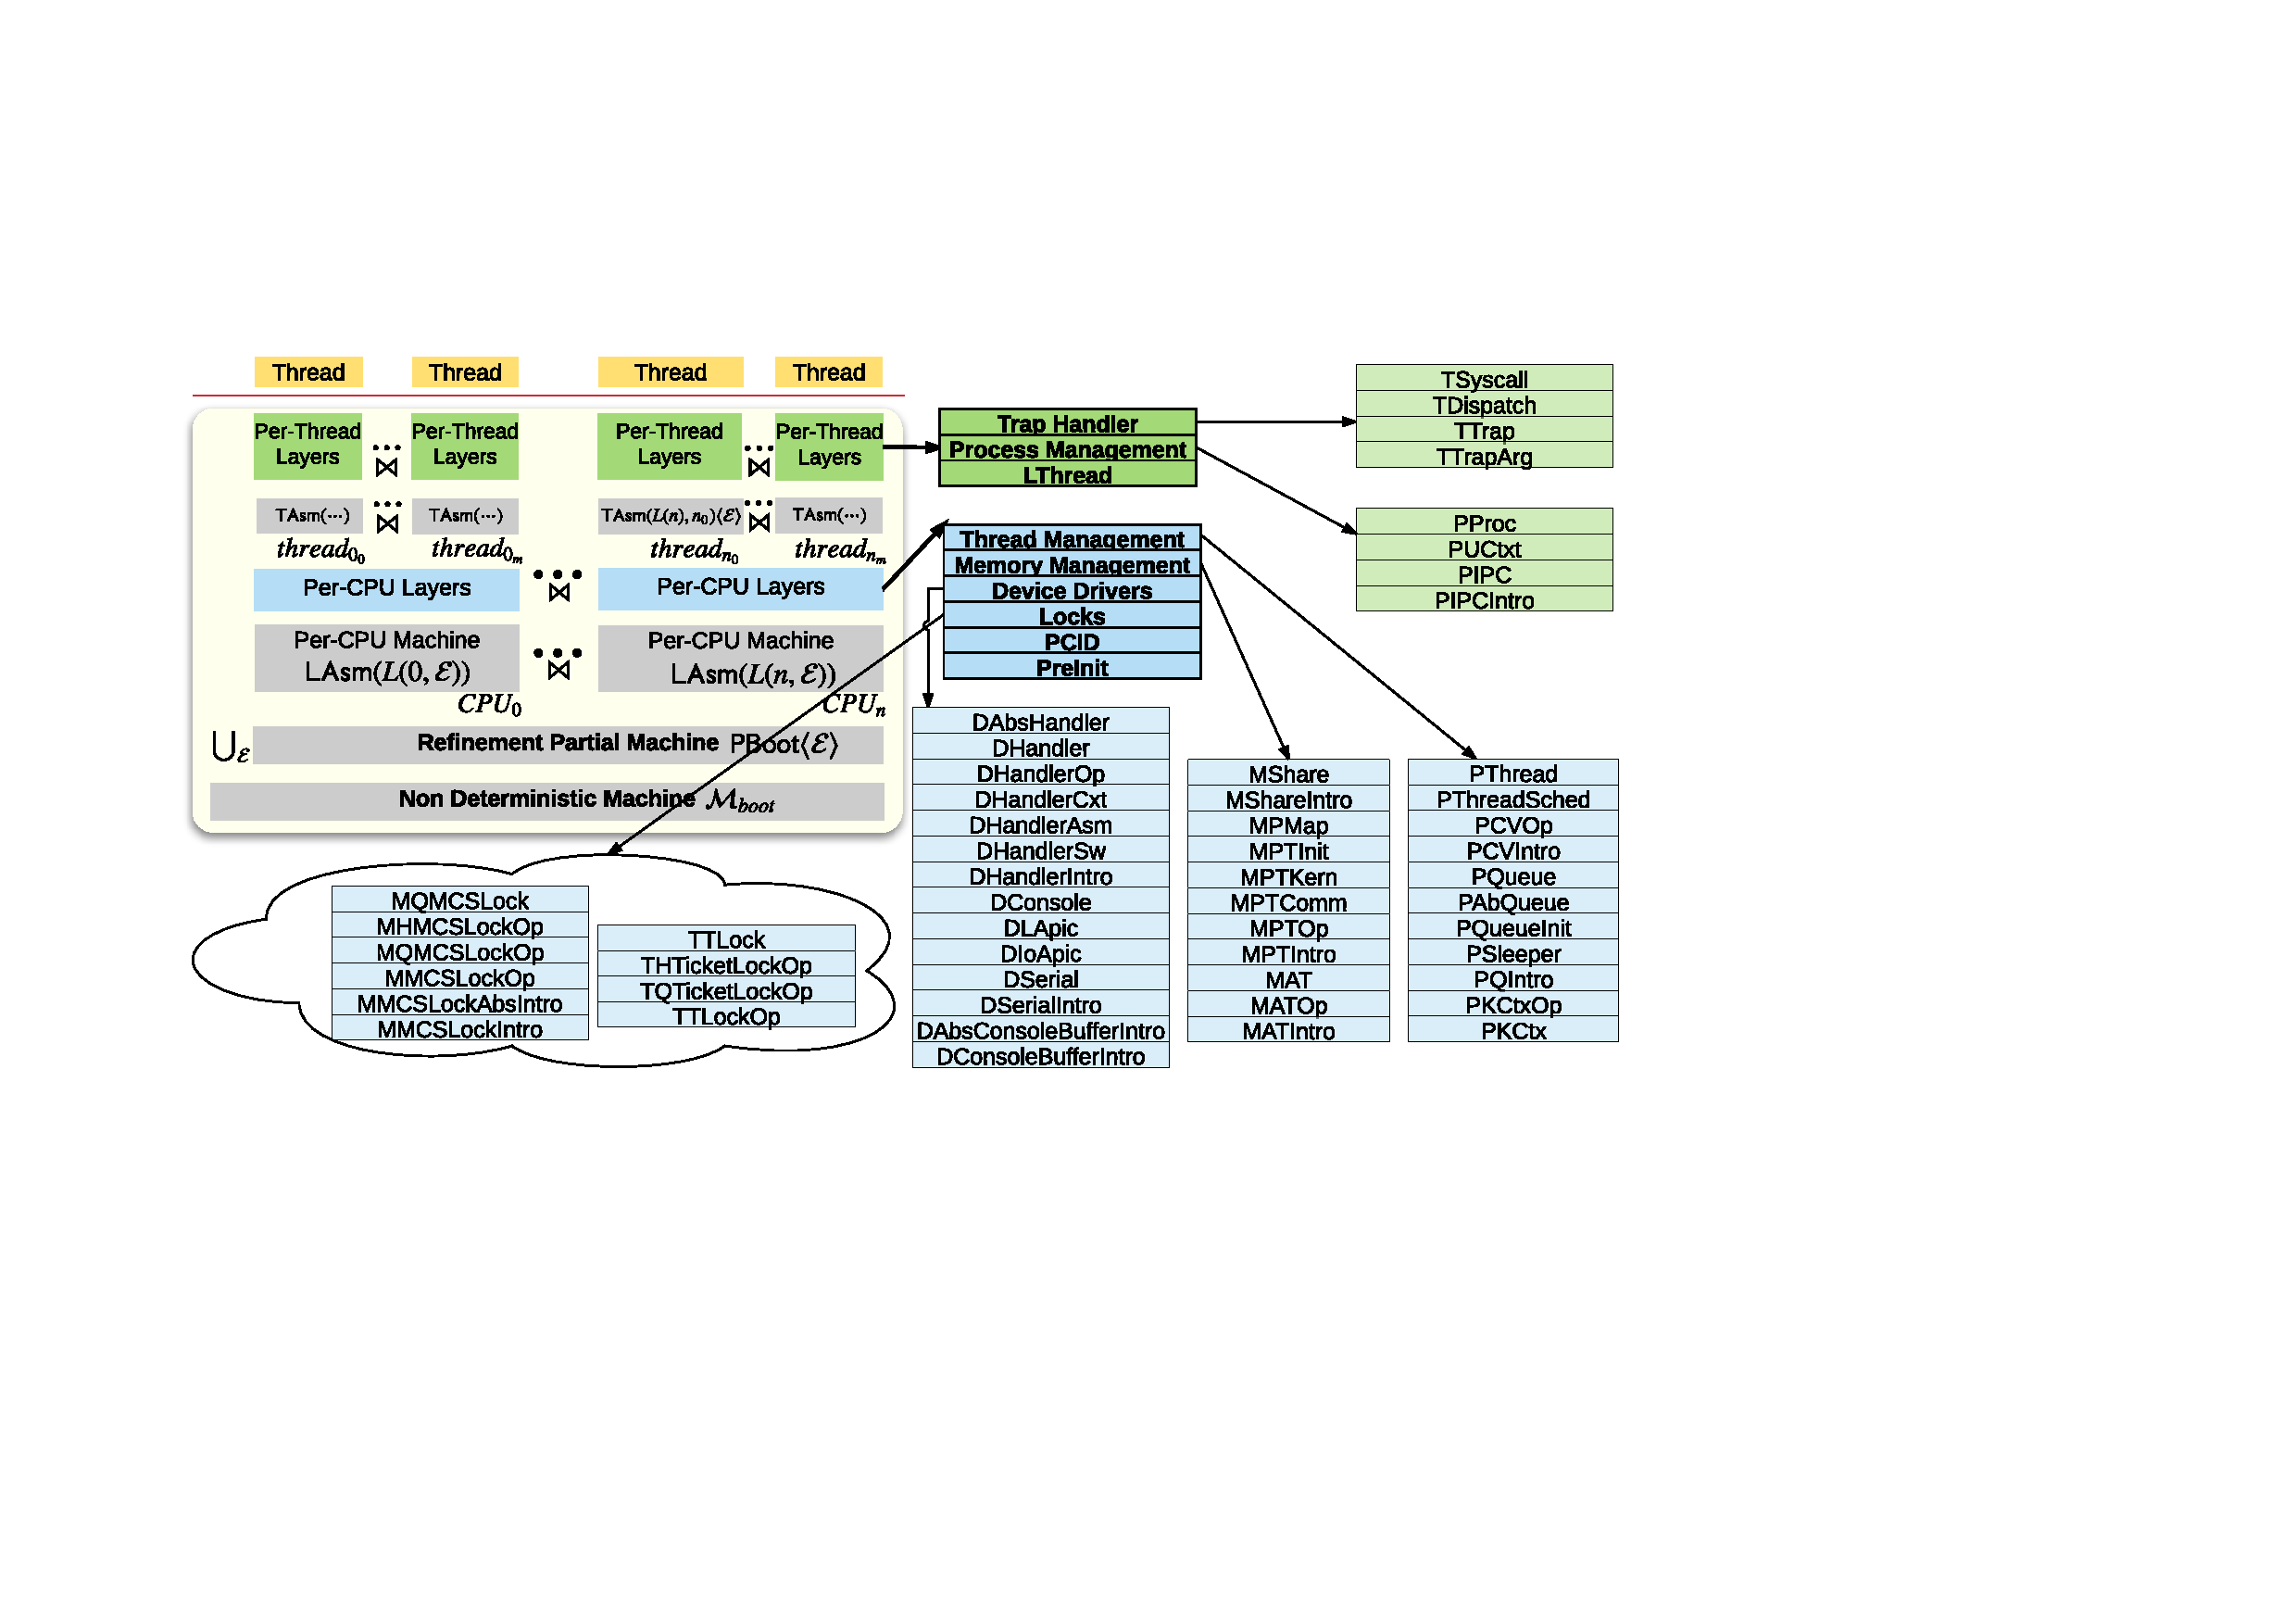
\includegraphics[scale=0.1]{figs/layer_diagram.png}
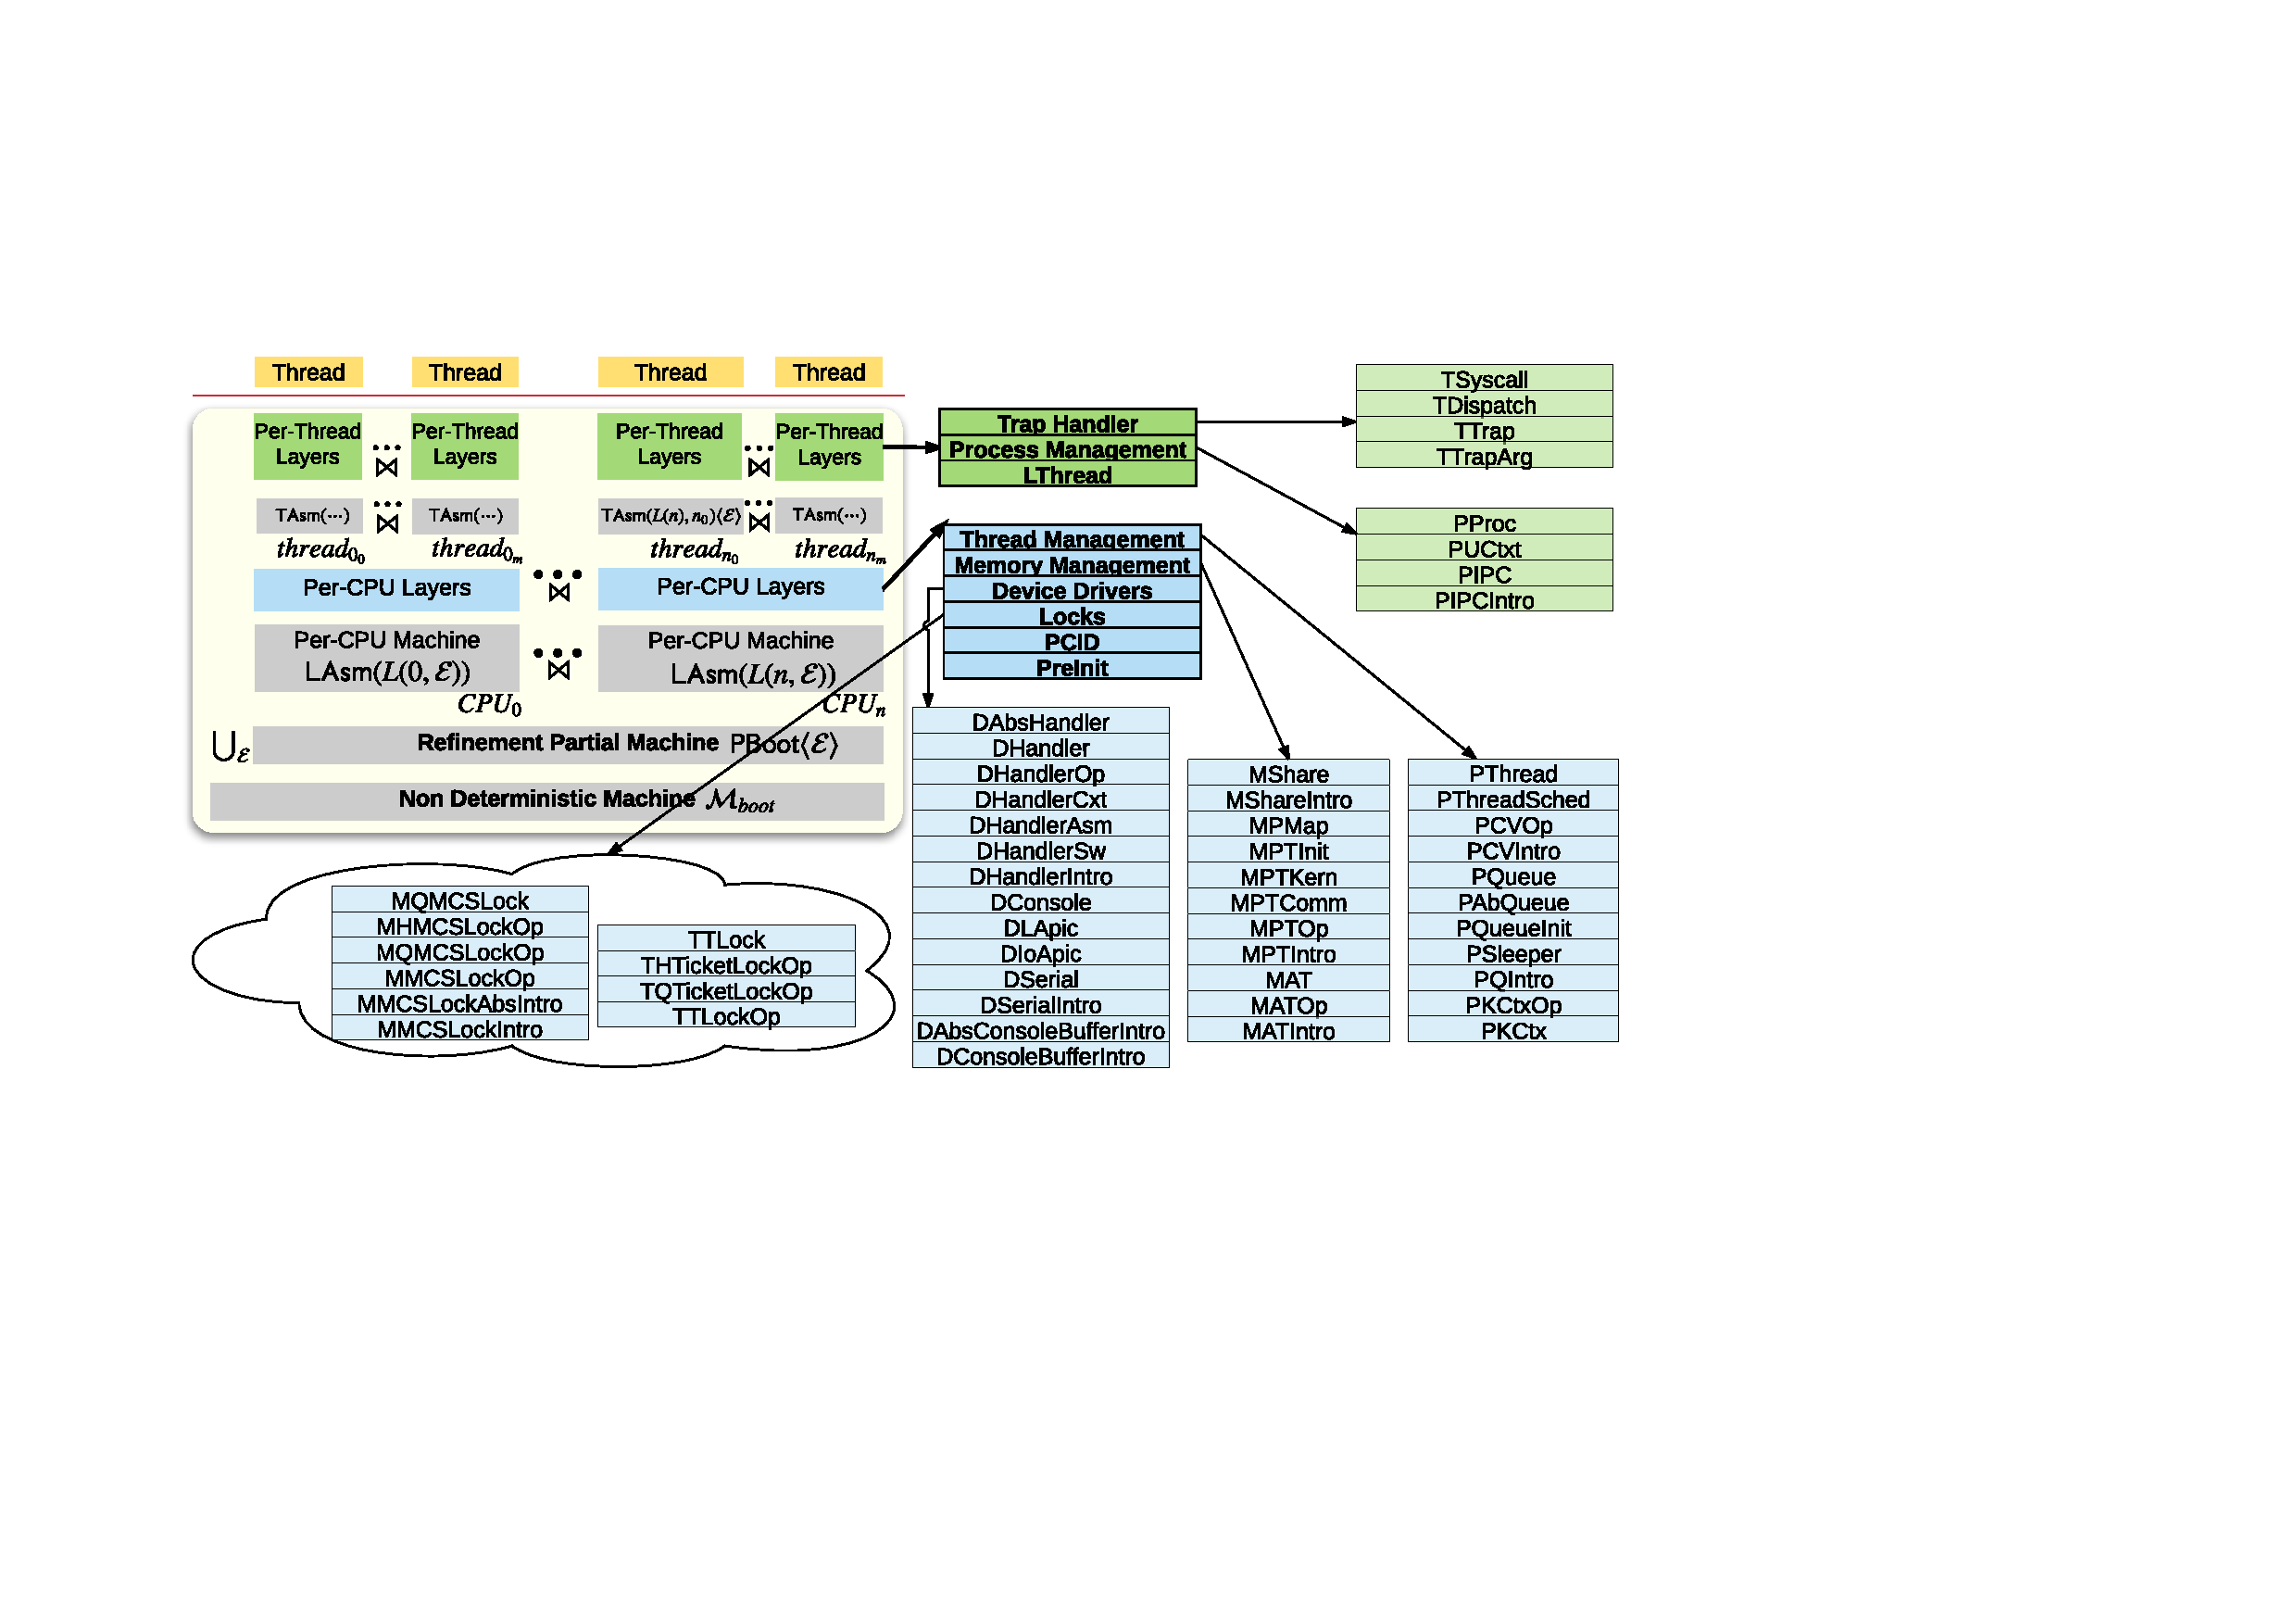
\includegraphics[width=1.0\textwidth]{figs/layer_diagram.pdf}
\vspace{-20pt}
\caption{Layer hierarchy of \cCTOS{} kernel}
\label{fig:layer_diagram}
\vspace{-10pt}
\end{figure*}

We demonstrate our new technology
by extending the \mCTOS{} single-core verified kernel \cite{dscal15} into a
concurrent kernel \cCTOS{} running on multi-core hardware.
In addition to all the concurrent objects described in Sec. \ref{sec:prog},
the kernel also implements an MCS lock \cite{mcs91}, paging-based dynamically
allocated virtual memory,
a synchronous inter-process communication (IPC) protocol implemented using the
queuing lock, and a shared-memory IPC protocol with a shared page.
Using the techniques and strategies presented in the paper, we have
successfully specified and verified the \cCTOS{} kernel in the Coq proof assistant.

Fig.~\ref{fig:layer_diagram} shows the layer hierarchy of  \cCTOS{}.
The gray boxes denote machine models, on top of which the
per-CPU (blue) and per-thread (yellow) layers are built. Orange boxes
are user threads.

The bottom-left portion of the figure illustrates the contextual refinement
among machine models, where we gradually turn the nondeterministic
multicore machine model with arbitrary interleavings
among different processors into a CPU-local machine model that is parameterized
over the behaviors of other processors,
where the switch points only appear at shared operations. This new machine
model allows us to reason about programs running on different processors locally,
and later compose them formally to reason about the whole program.

On top of this abstract machine model, the code of the concurrent kernel is specified and 
verified through 59 abstraction (logical) layers. For each CPU,
we introduce the atomic (ticket and MCS) spinlock objects following
the techniques presented in Sec.~\ref{sec:prog}.
On top of that, the device drivers running inside kernel are verified.
Then there are multiple layers used to introduce memory management units,
the thread context, atomic queue object, and scheduler methods (\cf Sec.~\ref{sec:prog}).
The \texttt{PThread} layer is the topmost layer built for a particular processor.
There, the scheduler primitives like \texttt{yield} and \texttt{sleep}
are specified in a small-step manner, similar to how they are implemented
in C and assembly. Their specifications do not follow the C calling conventions
and thus cannot be called by C code. Above \texttt{PThread}, we then build up the 
per-thread layers that support thread-local reasoning for each CPU.
We first introduce the layer \texttt{PHThread} which defines big-step semantics for
the scheduler primitives that can be invoked from the C level (\cf Sec.~\ref{sec:prog}).
Finally, above the \texttt{PHThread} layer, we verify the
IPC and trap handler modules.

The verified kernel source code (both C and assembly) is extracted using 
Coq's extraction mechanism. The C source code is then compiled by the
extracted verified compiler and merged with the extracted assembly source to
produce the final assembly source code for our verified concurrent kernel. 

\paragraph{Verification Effort and Lessons Learned}
Our team completed verification of the \cCTOS{} kernel in about 2 person years.
The layered approach is key to the scalability and feasibility of such a
large-scale verification effort.
One benefit of our approach is that
concrete and highly optimized (and thus complex) implementations can be abstracted
into much simpler logical specifications that are easier to reason about,
\eg, abstracting a queue implemented as a doubly-linked list into a simple logical list,
abstracting two-level page tables into a logical map from virtual addresses
to physical addresses with permissions, {\it etc}.
Besides this straightforward benefit, the layered approach shines in many other
aspects of complex system verification.

Layering allows us to perform incremental refinement of machine
  models. Real world CPUs are far from ideal for reasoning
purposes, so we abstract the realistic
machine model into a simpler one.
As indicated in Fig.~\ref{fig:layer_diagram}, the per-CPU layers are built on top
of an abstract machine model that supports CPU-local reasoning. Through
multiple contextual refinements, we have proved that the underlying
nondeterministic hardware machine model refines the abstract model. Furthermore, 
because each layer in our framework
is an abstract machine, we can do this not just at
the bottom, but at any point within the verification stack. For example, 
during the \cCTOS{} verification, we first abstract the two-level page table structure
in memory into a logical map from virtual addresses to physical addresses
with permissions. After doing this, we \emph{then} abstract the low level machine 
model that implements page-based virtual memory as described in the hardware 
manual into a simpler model using our abstract logical map.

Layering eases code verification in the concurrent setting.
It allows us to separate code verification from logical reasoning.
Concurrent program verification can be treated as a process of building
verified atomic objects. Each method of an atomic object is implemented using
locks and other atomic objects introduced at lower layers.
When we verify the function body of such a method, we first simply treat it as 
if it were sequential; this results in a non-atomic specification that allows
multiple events to occur. Then, through a separate contextual refinement
that does not involve any code verification, we abstract the environment
context to obtain a new, atomic specification generating only a single event.
In this way, we manage to cleanly separate concurrency reasoning 
(e.g., interleaved executions) from code verification.

\ignore{
{\it Layering facilitates the invariant preservation proof.}
Invariant preservation proofs represent one of the most expensive
components of large-scale verification projects \cite{klein2009sel4}.
They are expensive because they need to be proved not only locally, but
also for the global execution of the whole program. Additionally, many low 
level data manipulation functions temporarily break invariants and reestablish them
later. In our layered approach, every global in-memory data
structure refines one or more isolated abstract logical states in
higher layers. This results in automatic isolation guarantees, despite the
fact that underlying implementations at lower layers still manipulate pointers to
the data structure. Furthermore, each abstraction layer may have a different set
of invariants in our framework, so invariants are introduced incrementally.
For example, consider a queue implemented as a doubly-linked list in
memory. If we directly impose the invariant that the queue is always
well-formed, then we need to prove that no other pointer manipulation in the kernel 
breaks this invariant, while also dealing with the situation where low level 
code temporarily breaks but then reestablishes the invariant. 
Instead, we first abstract
the concrete implementation of the queue into a simple logical list, hiding
concrete pointer manipulation beneath abstract read/write primitives.
Then at higher layers, we gradually introduce and verify the
abstract \texttt{enqueue} and \texttt{dequeue} operations that utilize these
read/write primitives. The well-formedness invariant is only introduced at this 
layer where the \texttt{enqueue} and \texttt{dequeue} operations are atomic and 
all the lower level primitives are already hidden. 
}


\ignore{
\newman{Don't read further. Below are just some random sentences got cut from the OSDI version.}

Furthermore, note that we did not reach the current working solution
in one shot. We first spent about 3 person months developing an
unsuccessful version of the framework for composing multi-threaded
execution on a single CPU.  In that version, thread-local execution
was modeled using a \emph{time stamp} index into a global system
log. We eventually realized that the exact time stamps were too
cumbersome and revealed too much information about the underlying
implementation (\eg, the number of software yields within a function
body), so we spent another month developing a new system that uses
local logs (lists of events) instead.\ignore{ of time stamps, and the
  ability to shuffle and merge the events in the local logs to hide
  unnecessary nondeterminism or implementation details.}  Our initial
multicore machine model also did not work out very well when we
developed the multicore linking framework; we spent 3 person weeks to
improve the initial design through multiple iterations.  The main
challenge was finding the right invariants for the environment
context, such that we could successfully establish starvation-freedom.

\paragraph{Abstraction Layers}
\newman{I am gonna write some summary about the layered approach after I read
the overview section to see how much of the concepts are already covered.}
\begin{itemize}
\item Abstraction of data representation: doubly-linked list --> logical list
\item Stronger invariants
\item Abstraction of primitive specification: hiding log implementation by linking and merging events
\item Refinement of machine models: from a realistic machine model to an ideal machine model that is suitable for our reasoning purpose, e.g., change in machine/memory/interrupt model
\end{itemize}

The verification effort roughly falls into three categories: layer
design with specification and invariants, refinement proofs between
the layers, and verification of C and assembly code with respect to
the specifications. The time needed for each of the categories depends
largely on the layer.  For instance, at the boundary of physical and
virtual memory management (\texttt{MPTIntro}), almost all effort
is in the refinement proof, due to the proof for the refinement between
two completely different memory models. More effort went into the
refinement proof when we introduced the Intel \emph{virtual machine
memory model}, where we proved the refinement between the concrete
four level extended page table structure in memory and the abstract
mapping from the guest addresses to the host addresses.
In contrast, for the layer \texttt{MATOp},
which initializes physical memory allocation,
most of the time was spent on verifying
the non-trivial nested loops present in the C code,
while the refinement proofs were derived automatically. 

The proofs were facilitated by automation tools for C
code, layer design patterns, and tactics libraries developed in
recent years \cite{dscal15}. These tools have greatly
reduced the amount of work needed to verify extensions of the kernel.


Verification not only
should not hinder application of similar performance optimizations,
but instead provide a safety net for more aggressive optimizations, if
it is required for application scenarios of the kernel we have in
mind.
}
